%! \usetikzlibrary{decorations.pathreplacing,decorations.pathmorphing}
\usetikzlibrary{decorations.pathmorphing,decorations.markings}
\providecommand{\ket}[1]{\left|#1\right\rangle}
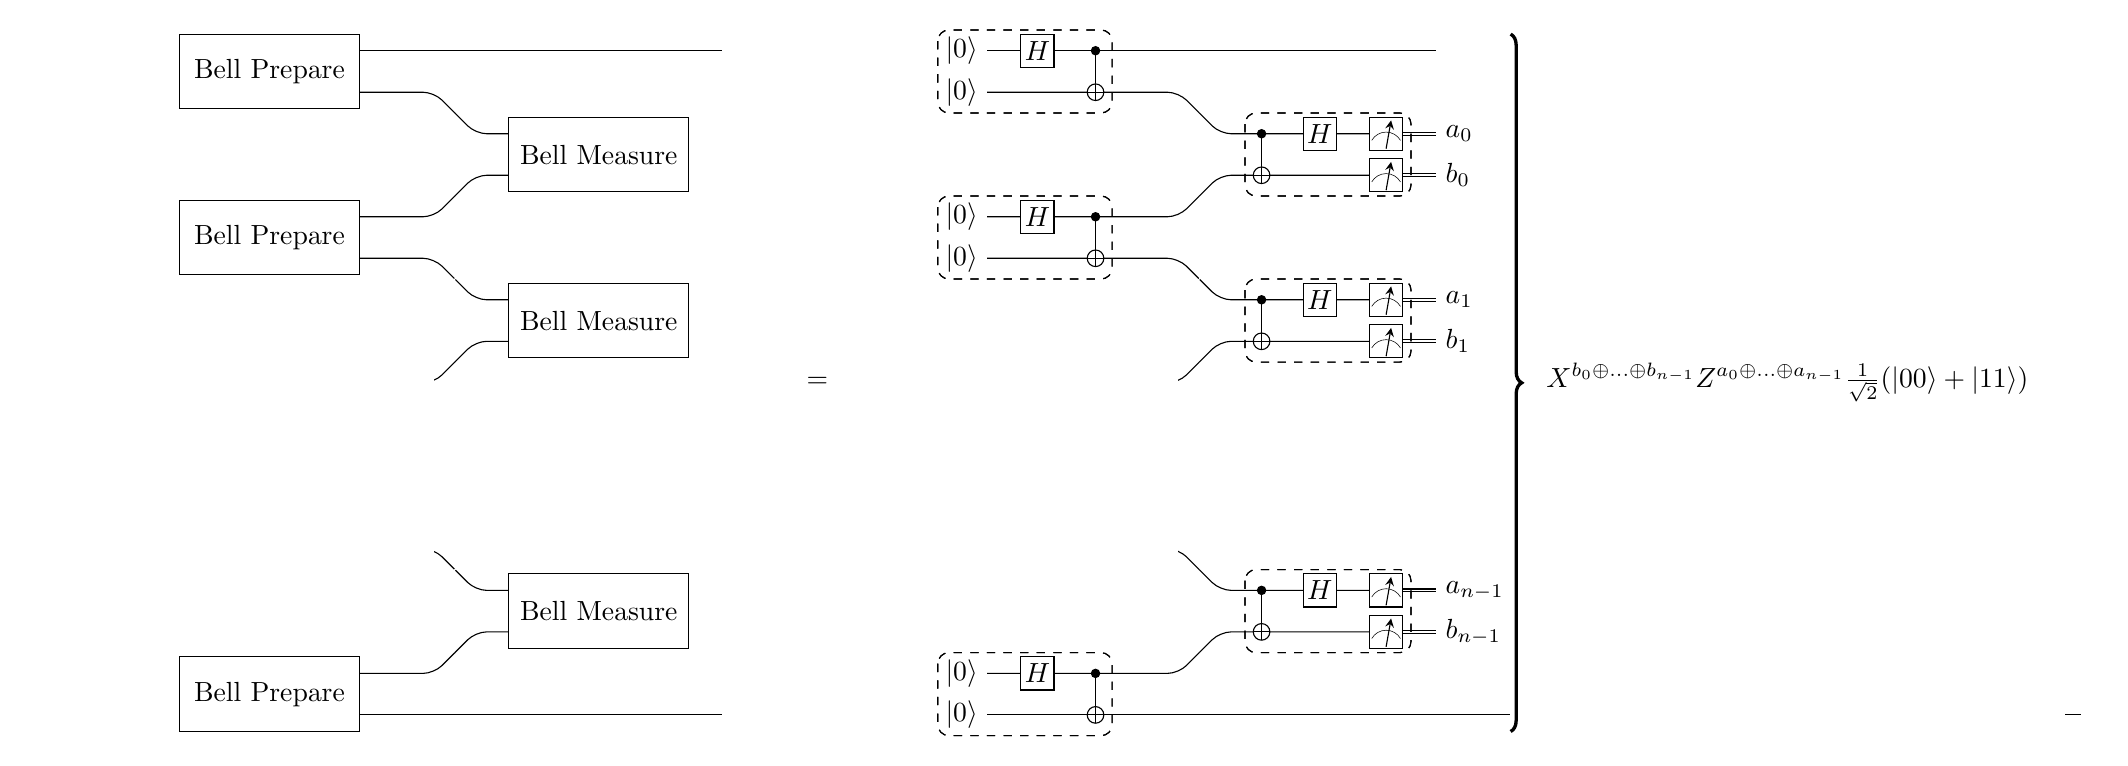
\begin{tikzpicture}[scale=1.000000,x=1pt,y=1pt]
\filldraw[color=white] (0.000000, -7.500000) rectangle (735.000000, 247.500000);
% Drawing wires
% Line 11: x W {} {} {\ket{0}} {}
\draw[color=white] (21.000000,240.000000) -- (80.500000,240.000000);
\draw[color=black] (80.500000,240.000000) -- (140.000000,240.000000);
\draw[color=black] (140.000000,240.000000) -- (147.500000,240.000000);
\draw[color=black] (147.500000,240.000000) -- (155.000000,240.000000);
\draw[color=black] (155.000000,240.000000) -- (251.500000,240.000000);
\draw[color=black] (332.500000,240.000000) -- (409.000000,240.000000);
\draw[color=black] (409.000000,240.000000) -- (416.500000,240.000000);
\draw[color=black] (416.500000,240.000000) -- (424.000000,240.000000);
\draw[color=black] (424.000000,240.000000) -- (509.500000,240.000000);
% Line 12: y W {} {} {\ket{0}} {a_0}
\draw[color=white] (21.000000,225.000000) -- (80.500000,225.000000);
\draw[color=black,rounded corners=4.000000pt] (80.500000,225.000000) -- (140.000000,225.000000) -- (147.500000,217.500000);
\draw[color=black,rounded corners=4.000000pt] (147.500000,217.500000) -- (155.000000,210.000000) -- (199.500000,210.000000);
\draw[color=white] (199.500000,210.000000) -- (251.500000,210.000000);
\draw[color=black,rounded corners=4.000000pt] (332.500000,225.000000) -- (409.000000,225.000000) -- (416.500000,217.500000);
\draw[color=black,rounded corners=4.000000pt] (416.500000,217.500000) -- (424.000000,210.000000) -- (484.000000,210.000000);
\draw[color=black] (484.000000,209.500000) -- (509.500000,209.500000);
\draw[color=black] (484.000000,210.500000) -- (509.500000,210.500000);
% Line 13: buf1 W
\draw[color=white] (13.500000,210.000000) -- (28.500000,210.000000);
% Line 14: buf2 W
\draw[color=white] (13.500000,195.000000) -- (28.500000,195.000000);
% Line 15: z W {} {} {\ket{0}} {b_0}
\draw[color=white] (21.000000,180.000000) -- (80.500000,180.000000);
\draw[color=black,rounded corners=4.000000pt] (80.500000,180.000000) -- (140.000000,180.000000) -- (147.500000,187.500000);
\draw[color=black,rounded corners=4.000000pt] (147.500000,187.500000) -- (155.000000,195.000000) -- (199.500000,195.000000);
\draw[color=white] (199.500000,195.000000) -- (251.500000,195.000000);
\draw[color=black,rounded corners=4.000000pt] (332.500000,180.000000) -- (409.000000,180.000000) -- (416.500000,187.500000);
\draw[color=black,rounded corners=4.000000pt] (416.500000,187.500000) -- (424.000000,195.000000) -- (484.000000,195.000000);
\draw[color=black] (484.000000,194.500000) -- (509.500000,194.500000);
\draw[color=black] (484.000000,195.500000) -- (509.500000,195.500000);
% Line 16: w W {} {} {\ket{0}} {a_1}
\draw[color=white] (21.000000,165.000000) -- (80.500000,165.000000);
\draw[color=black,rounded corners=4.000000pt] (80.500000,165.000000) -- (140.000000,165.000000) -- (147.500000,157.500000);
\draw[color=black,rounded corners=4.000000pt] (147.500000,157.500000) -- (155.000000,150.000000) -- (199.500000,150.000000);
\draw[color=white] (199.500000,150.000000) -- (251.500000,150.000000);
\draw[color=black,rounded corners=4.000000pt] (332.500000,165.000000) -- (409.000000,165.000000) -- (416.500000,157.500000);
\draw[color=black,rounded corners=4.000000pt] (416.500000,157.500000) -- (424.000000,150.000000) -- (484.000000,150.000000);
\draw[color=black] (484.000000,149.500000) -- (509.500000,149.500000);
\draw[color=black] (484.000000,150.500000) -- (509.500000,150.500000);
% Line 17: a W {} {} {} {}
\draw[color=white,rounded corners=4.000000pt] (21.000000,150.000000) -- (140.000000,150.000000) -- (147.500000,157.500000);
\draw[color=white,rounded corners=4.000000pt] (147.500000,157.500000) -- (155.000000,165.000000) -- (298.000000,165.000000) -- (305.500000,157.500000);
\draw[color=white,rounded corners=4.000000pt] (305.500000,157.500000) -- (313.000000,150.000000) -- (332.500000,150.000000);
\draw[color=white,rounded corners=4.000000pt] (332.500000,150.000000) -- (409.000000,150.000000) -- (416.500000,157.500000);
\draw[color=white,rounded corners=4.000000pt] (416.500000,157.500000) -- (424.000000,165.000000) -- (735.000000,165.000000);
% Line 18: b W {} {} {} {}
\draw[color=white,rounded corners=4.000000pt] (21.000000,135.000000) -- (140.000000,135.000000) -- (147.500000,127.500000);
\draw[color=white,rounded corners=4.000000pt] (147.500000,127.500000) -- (155.000000,120.000000) -- (251.500000,120.000000);
\draw[color=white,rounded corners=4.000000pt] (332.500000,135.000000) -- (409.000000,135.000000) -- (416.500000,127.500000);
\draw[color=white,rounded corners=4.000000pt] (416.500000,127.500000) -- (424.000000,120.000000) -- (509.500000,120.000000);
% Line 19: c W {} {} {} {b_1}
\draw[color=black,rounded corners=4.000000pt] (132.500000,120.000000) -- (140.000000,120.000000) -- (147.500000,127.500000);
\draw[color=black,rounded corners=4.000000pt] (147.500000,127.500000) -- (155.000000,135.000000) -- (199.500000,135.000000);
\draw[color=white] (199.500000,135.000000) -- (251.500000,135.000000);
\draw[color=black,rounded corners=4.000000pt] (401.500000,120.000000) -- (409.000000,120.000000) -- (416.500000,127.500000);
\draw[color=black,rounded corners=4.000000pt] (416.500000,127.500000) -- (424.000000,135.000000) -- (484.000000,135.000000);
\draw[color=black] (484.000000,134.500000) -- (509.500000,134.500000);
\draw[color=black] (484.000000,135.500000) -- (509.500000,135.500000);
% Line 20: buf3 W color=white
\draw[color=white] (0.000000,105.000000) -- (140.000000,105.000000);
\draw[color=white] (140.000000,105.000000) -- (147.500000,105.000000);
\draw[color=white] (147.500000,105.000000) -- (155.000000,105.000000);
\draw[color=white] (155.000000,105.000000) -- (298.000000,105.000000);
\draw[color=white] (298.000000,105.000000) -- (305.500000,105.000000);
\draw[color=white] (305.500000,105.000000) -- (313.000000,105.000000);
\draw[color=white] (313.000000,105.000000) -- (409.000000,105.000000);
\draw[color=white] (409.000000,105.000000) -- (416.500000,105.000000);
\draw[color=white] (416.500000,105.000000) -- (424.000000,105.000000);
\draw[color=white] (424.000000,105.000000) -- (735.000000,105.000000);
% Line 21: buf4 W color=white
\draw[color=white] (0.000000,90.000000) -- (140.000000,90.000000);
\draw[color=white] (140.000000,90.000000) -- (147.500000,90.000000);
\draw[color=white] (147.500000,90.000000) -- (155.000000,90.000000);
\draw[color=white] (155.000000,90.000000) -- (298.000000,90.000000);
\draw[color=white] (298.000000,90.000000) -- (305.500000,90.000000);
\draw[color=white] (305.500000,90.000000) -- (313.000000,90.000000);
\draw[color=white] (313.000000,90.000000) -- (409.000000,90.000000);
\draw[color=white] (409.000000,90.000000) -- (416.500000,90.000000);
\draw[color=white] (416.500000,90.000000) -- (424.000000,90.000000);
\draw[color=white] (424.000000,90.000000) -- (735.000000,90.000000);
% Line 22: buf5 W color=white
\draw[color=white] (0.000000,75.000000) -- (140.000000,75.000000);
\draw[color=white] (140.000000,75.000000) -- (147.500000,75.000000);
\draw[color=white] (147.500000,75.000000) -- (155.000000,75.000000);
\draw[color=white] (155.000000,75.000000) -- (298.000000,75.000000);
\draw[color=white] (298.000000,75.000000) -- (305.500000,75.000000);
\draw[color=white] (305.500000,75.000000) -- (313.000000,75.000000);
\draw[color=white] (313.000000,75.000000) -- (409.000000,75.000000);
\draw[color=white] (409.000000,75.000000) -- (416.500000,75.000000);
\draw[color=white] (416.500000,75.000000) -- (424.000000,75.000000);
\draw[color=white] (424.000000,75.000000) -- (735.000000,75.000000);
% Line 24: d W color=white {} {} {a_{n-1}}
\draw[color=black,rounded corners=4.000000pt] (132.500000,60.000000) -- (140.000000,60.000000) -- (147.500000,52.500000);
\draw[color=black,rounded corners=4.000000pt] (147.500000,52.500000) -- (155.000000,45.000000) -- (199.500000,45.000000);
\draw[color=white,rounded corners=4.000000pt] (199.500000,45.000000) -- (298.000000,45.000000) -- (305.500000,52.500000);
\draw[color=white,rounded corners=4.000000pt] (305.500000,52.500000) -- (313.000000,60.000000) -- (401.500000,60.000000);
\draw[color=black,rounded corners=4.000000pt] (401.500000,60.000000) -- (409.000000,60.000000) -- (416.500000,52.500000);
\draw[color=black,rounded corners=4.000000pt] (416.500000,52.500000) -- (424.000000,45.000000) -- (484.000000,45.000000);
\draw[color=black] (484.000000,44.500000) -- (509.500000,44.500000);
\draw[color=black] (484.000000,45.500000) -- (509.500000,45.500000);
% Line 25: e W color=white
\draw[color=white,rounded corners=4.000000pt] (0.000000,45.000000) -- (140.000000,45.000000) -- (147.500000,52.500000);
\draw[color=white,rounded corners=4.000000pt] (147.500000,52.500000) -- (155.000000,60.000000) -- (251.500000,60.000000);
% Line 26: f W color=white
\draw[color=white,rounded corners=4.000000pt] (21.000000,30.000000) -- (140.000000,30.000000) -- (147.500000,22.500000);
\draw[color=white,rounded corners=4.000000pt] (147.500000,22.500000) -- (155.000000,15.000000) -- (251.500000,15.000000);
\draw[color=white,rounded corners=4.000000pt] (332.500000,30.000000) -- (409.000000,30.000000) -- (416.500000,22.500000);
\draw[color=white,rounded corners=4.000000pt] (416.500000,22.500000) -- (424.000000,15.000000) -- (509.500000,15.000000);
% Line 27: g W color=white {} {} {\ket{0}} {b_{n-1}}
\draw[color=white] (21.000000,15.000000) -- (80.500000,15.000000);
\draw[color=black,rounded corners=4.000000pt] (80.500000,15.000000) -- (140.000000,15.000000) -- (147.500000,22.500000);
\draw[color=black,rounded corners=4.000000pt] (147.500000,22.500000) -- (155.000000,30.000000) -- (199.500000,30.000000);
\draw[color=white] (199.500000,30.000000) -- (251.500000,30.000000);
\draw[color=black,rounded corners=4.000000pt] (332.500000,15.000000) -- (409.000000,15.000000) -- (416.500000,22.500000);
\draw[color=black,rounded corners=4.000000pt] (416.500000,22.500000) -- (424.000000,30.000000) -- (484.000000,30.000000);
\draw[color=black] (484.000000,29.500000) -- (509.500000,29.500000);
\draw[color=black] (484.000000,30.500000) -- (509.500000,30.500000);
% Line 28: h W color=white {} {} {\ket{0}}
\draw[color=white] (0.000000,0.000000) -- (80.500000,0.000000);
\draw[color=black] (80.500000,0.000000) -- (140.000000,0.000000);
\draw[color=black] (140.000000,0.000000) -- (147.500000,0.000000);
\draw[color=black] (147.500000,0.000000) -- (155.000000,0.000000);
\draw[color=black] (155.000000,0.000000) -- (251.500000,0.000000);
\draw[color=black] (332.500000,0.000000) -- (409.000000,0.000000);
\draw[color=black] (409.000000,0.000000) -- (416.500000,0.000000);
\draw[color=black] (416.500000,0.000000) -- (424.000000,0.000000);
\draw[color=black] (424.000000,0.000000) -- (735.000000,0.000000);
\draw[color=white] (0.000000,0.000000) node[left] {${}$};
% Done with wires; drawing gates
% Line 33: x START x:color=white
\draw[color=white] (28.500000,240.000000) node[fill=white,left,minimum height=15.000000pt,minimum width=15.000000pt,inner sep=0pt] {\phantom{${}$}};
\draw[color=white] (28.500000,240.000000) node[left] {${}$};
% Line 34: y START y:color=white
\draw[color=white] (28.500000,225.000000) node[fill=white,left,minimum height=15.000000pt,minimum width=15.000000pt,inner sep=0pt] {\phantom{${}$}};
\draw[color=white] (28.500000,225.000000) node[left] {${}$};
% Line 35: z START z:color=white
\draw[color=white] (28.500000,180.000000) node[fill=white,left,minimum height=15.000000pt,minimum width=15.000000pt,inner sep=0pt] {\phantom{${}$}};
\draw[color=white] (28.500000,180.000000) node[left] {${}$};
% Line 36: w START w:color=white
\draw[color=white] (28.500000,165.000000) node[fill=white,left,minimum height=15.000000pt,minimum width=15.000000pt,inner sep=0pt] {\phantom{${}$}};
\draw[color=white] (28.500000,165.000000) node[left] {${}$};
% Line 37: buf1 START buf1:color=white; buf1 END
% Line 37: buf1 START buf1:color=white; buf1 END
% Line 38: buf2 START buf2:color=white; buf2 END
% Line 38: buf2 START buf2:color=white; buf2 END
% Line 39: a START a:color=white
\draw[color=white] (28.500000,150.000000) node[fill=white,left,minimum height=15.000000pt,minimum width=15.000000pt,inner sep=0pt] {\phantom{${}$}};
\draw[color=white] (28.500000,150.000000) node[left] {${}$};
% Line 40: b START b:color=white
\draw[color=white] (28.500000,135.000000) node[fill=white,left,minimum height=15.000000pt,minimum width=15.000000pt,inner sep=0pt] {\phantom{${}$}};
\draw[color=white] (28.500000,135.000000) node[left] {${}$};
% Line 41: f START f:color=white
% Line 42: g START g:color=white
\draw[color=white] (28.500000,15.000000) node[fill=white,left,minimum height=15.000000pt,minimum width=15.000000pt,inner sep=0pt] {\phantom{${}$}};
\draw[color=white] (28.500000,15.000000) node[left] {${}$};
% Line 46: x y G {Bell Prepare} width=65 x:color=black y:color=black
\draw (80.500000,240.000000) -- (80.500000,225.000000);
\begin{scope}
\draw[fill=white] (80.500000, 232.500000) +(-45.000000:45.961941pt and 19.091883pt) -- +(45.000000:45.961941pt and 19.091883pt) -- +(135.000000:45.961941pt and 19.091883pt) -- +(225.000000:45.961941pt and 19.091883pt) -- cycle;
\clip (80.500000, 232.500000) +(-45.000000:45.961941pt and 19.091883pt) -- +(45.000000:45.961941pt and 19.091883pt) -- +(135.000000:45.961941pt and 19.091883pt) -- +(225.000000:45.961941pt and 19.091883pt) -- cycle;
\draw (80.500000, 232.500000) node {{Bell Prepare}};
\end{scope}
% Line 47: z w G {Bell Prepare} width=65 z:color=black w:color=black
\draw (80.500000,180.000000) -- (80.500000,165.000000);
\begin{scope}
\draw[fill=white] (80.500000, 172.500000) +(-45.000000:45.961941pt and 19.091883pt) -- +(45.000000:45.961941pt and 19.091883pt) -- +(135.000000:45.961941pt and 19.091883pt) -- +(225.000000:45.961941pt and 19.091883pt) -- cycle;
\clip (80.500000, 172.500000) +(-45.000000:45.961941pt and 19.091883pt) -- +(45.000000:45.961941pt and 19.091883pt) -- +(135.000000:45.961941pt and 19.091883pt) -- +(225.000000:45.961941pt and 19.091883pt) -- cycle;
\draw (80.500000, 172.500000) node {{Bell Prepare}};
\end{scope}
% Line 48: g h G {Bell Prepare} width=65 h:color=black g:color=black
\draw (80.500000,15.000000) -- (80.500000,0.000000);
\begin{scope}
\draw[fill=white] (80.500000, 7.500000) +(-45.000000:45.961941pt and 19.091883pt) -- +(45.000000:45.961941pt and 19.091883pt) -- +(135.000000:45.961941pt and 19.091883pt) -- +(225.000000:45.961941pt and 19.091883pt) -- cycle;
\clip (80.500000, 7.500000) +(-45.000000:45.961941pt and 19.091883pt) -- +(45.000000:45.961941pt and 19.091883pt) -- +(135.000000:45.961941pt and 19.091883pt) -- +(225.000000:45.961941pt and 19.091883pt) -- cycle;
\draw (80.500000, 7.500000) node {{Bell Prepare}};
\end{scope}
% Line 51: c START c:color=black; d START d:color=black; x buf1 y z buf2 a w c b e d g f h PERMUTE
\draw[color=black] (140.000000,120.000000) node[fill=white,left,minimum height=15.000000pt,minimum width=15.000000pt,inner sep=0pt] {\phantom{${}$}};
\draw[color=black] (140.000000,120.000000) node[left] {${}$};
% Line 51: c START c:color=black; d START d:color=black; x buf1 y z buf2 a w c b e d g f h PERMUTE
\draw[color=black] (140.000000,60.000000) node[fill=white,left,minimum height=15.000000pt,minimum width=15.000000pt,inner sep=0pt] {\phantom{${}$}};
\draw[color=black] (140.000000,60.000000) node[left] {${}$};
% Line 51: c START c:color=black; d START d:color=black; x buf1 y z buf2 a w c b e d g f h PERMUTE
% Line 53: y z G {Bell Measure} width=65 z:color=white y:color=white
\draw (199.500000,210.000000) -- (199.500000,195.000000);
\begin{scope}
\draw[fill=white] (199.500000, 202.500000) +(-45.000000:45.961941pt and 19.091883pt) -- +(45.000000:45.961941pt and 19.091883pt) -- +(135.000000:45.961941pt and 19.091883pt) -- +(225.000000:45.961941pt and 19.091883pt) -- cycle;
\clip (199.500000, 202.500000) +(-45.000000:45.961941pt and 19.091883pt) -- +(45.000000:45.961941pt and 19.091883pt) -- +(135.000000:45.961941pt and 19.091883pt) -- +(225.000000:45.961941pt and 19.091883pt) -- cycle;
\draw (199.500000, 202.500000) node {{Bell Measure}};
\end{scope}
% Line 54: w c G {Bell Measure} width=65 w:color=white c:color=white
\draw (199.500000,150.000000) -- (199.500000,135.000000);
\begin{scope}
\draw[fill=white] (199.500000, 142.500000) +(-45.000000:45.961941pt and 19.091883pt) -- +(45.000000:45.961941pt and 19.091883pt) -- +(135.000000:45.961941pt and 19.091883pt) -- +(225.000000:45.961941pt and 19.091883pt) -- cycle;
\clip (199.500000, 142.500000) +(-45.000000:45.961941pt and 19.091883pt) -- +(45.000000:45.961941pt and 19.091883pt) -- +(135.000000:45.961941pt and 19.091883pt) -- +(225.000000:45.961941pt and 19.091883pt) -- cycle;
\draw (199.500000, 142.500000) node {{Bell Measure}};
\end{scope}
% Line 55: g d G {Bell Measure} width=65 d:color=white g:color=white
\draw (199.500000,45.000000) -- (199.500000,30.000000);
\begin{scope}
\draw[fill=white] (199.500000, 37.500000) +(-45.000000:45.961941pt and 19.091883pt) -- +(45.000000:45.961941pt and 19.091883pt) -- +(135.000000:45.961941pt and 19.091883pt) -- +(225.000000:45.961941pt and 19.091883pt) -- cycle;
\clip (199.500000, 37.500000) +(-45.000000:45.961941pt and 19.091883pt) -- +(45.000000:45.961941pt and 19.091883pt) -- +(135.000000:45.961941pt and 19.091883pt) -- +(225.000000:45.961941pt and 19.091883pt) -- cycle;
\draw (199.500000, 37.500000) node {{Bell Measure}};
\end{scope}
% Line 60: x y z w c b e g f h END
\draw[color=black] (244.000000,240.000000) node[fill=white,right,minimum height=15.000000pt,minimum width=15.000000pt,inner sep=0pt] {\phantom{${}$}};
\draw[color=black] (244.000000,240.000000) node[right] {${}$};
\draw[color=white] (244.000000,210.000000) node[fill=white,right,minimum height=15.000000pt,minimum width=15.000000pt,inner sep=0pt] {\phantom{${}$}};
\draw[color=white] (244.000000,210.000000) node[right] {${}$};
\draw[color=white] (244.000000,195.000000) node[fill=white,right,minimum height=15.000000pt,minimum width=15.000000pt,inner sep=0pt] {\phantom{${}$}};
\draw[color=white] (244.000000,195.000000) node[right] {${}$};
\draw[color=white] (244.000000,150.000000) node[fill=white,right,minimum height=15.000000pt,minimum width=15.000000pt,inner sep=0pt] {\phantom{${}$}};
\draw[color=white] (244.000000,150.000000) node[right] {${}$};
\draw[color=white] (244.000000,135.000000) node[fill=white,right,minimum height=15.000000pt,minimum width=15.000000pt,inner sep=0pt] {\phantom{${}$}};
\draw[color=white] (244.000000,135.000000) node[right] {${}$};
\draw[color=white] (244.000000,120.000000) node[fill=white,right,minimum height=15.000000pt,minimum width=15.000000pt,inner sep=0pt] {\phantom{${}$}};
\draw[color=white] (244.000000,120.000000) node[right] {${}$};
\draw[color=white] (244.000000,30.000000) node[fill=white,right,minimum height=15.000000pt,minimum width=15.000000pt,inner sep=0pt] {\phantom{${}$}};
\draw[color=white] (244.000000,30.000000) node[right] {${}$};
\draw[color=black] (244.000000,0.000000) node[fill=white,right,minimum height=15.000000pt,minimum width=15.000000pt,inner sep=0pt] {\phantom{${}$}};
\draw[color=black] (244.000000,0.000000) node[right] {${}$};
% Line 62: =
\draw[fill=white,color=white] (271.000000, -6.000000) rectangle (286.000000, 246.000000);
\draw (278.500000, 120.000000) node {$=$};
% Line 64: x y buf1 buf2 z w a b c d e f g h PERMUTE
% Line 66: x START x:color=black
\draw[color=black] (340.000000,240.000000) node[fill=white,left,minimum height=15.000000pt,minimum width=15.000000pt,inner sep=0pt] {\phantom{${\ket{0}}$}};
\draw[color=black] (340.000000,240.000000) node[left] {${\ket{0}}$};
% Line 67: y START y:color=black
\draw[color=black] (340.000000,225.000000) node[fill=white,left,minimum height=15.000000pt,minimum width=15.000000pt,inner sep=0pt] {\phantom{${\ket{0}}$}};
\draw[color=black] (340.000000,225.000000) node[left] {${\ket{0}}$};
% Line 68: z START z:color=black
\draw[color=black] (340.000000,180.000000) node[fill=white,left,minimum height=15.000000pt,minimum width=15.000000pt,inner sep=0pt] {\phantom{${\ket{0}}$}};
\draw[color=black] (340.000000,180.000000) node[left] {${\ket{0}}$};
% Line 69: w START w:color=black
\draw[color=black] (340.000000,165.000000) node[fill=white,left,minimum height=15.000000pt,minimum width=15.000000pt,inner sep=0pt] {\phantom{${\ket{0}}$}};
\draw[color=black] (340.000000,165.000000) node[left] {${\ket{0}}$};
% Line 70: a START a:color=white
\draw[color=white] (340.000000,150.000000) node[fill=white,left,minimum height=15.000000pt,minimum width=15.000000pt,inner sep=0pt] {\phantom{${}$}};
\draw[color=white] (340.000000,150.000000) node[left] {${}$};
% Line 71: b START b:color=white
\draw[color=white] (340.000000,135.000000) node[fill=white,left,minimum height=15.000000pt,minimum width=15.000000pt,inner sep=0pt] {\phantom{${}$}};
\draw[color=white] (340.000000,135.000000) node[left] {${}$};
% Line 72: f START f:color=white
% Line 73: g START g:color=black
\draw[color=black] (340.000000,15.000000) node[fill=white,left,minimum height=15.000000pt,minimum width=15.000000pt,inner sep=0pt] {\phantom{${\ket{0}}$}};
\draw[color=black] (340.000000,15.000000) node[left] {${\ket{0}}$};
% Line 74: h START h:color=black
\draw[color=black] (340.000000,0.000000) node[fill=white,left,minimum height=15.000000pt,minimum width=15.000000pt,inner sep=0pt] {\phantom{${\ket{0}}$}};
\draw[color=black] (340.000000,0.000000) node[left] {${\ket{0}}$};
% Line 76: x G $H$
\begin{scope}
\draw[fill=white] (358.000000, 240.000000) +(-45.000000:8.485281pt and 8.485281pt) -- +(45.000000:8.485281pt and 8.485281pt) -- +(135.000000:8.485281pt and 8.485281pt) -- +(225.000000:8.485281pt and 8.485281pt) -- cycle;
\clip (358.000000, 240.000000) +(-45.000000:8.485281pt and 8.485281pt) -- +(45.000000:8.485281pt and 8.485281pt) -- +(135.000000:8.485281pt and 8.485281pt) -- +(225.000000:8.485281pt and 8.485281pt) -- cycle;
\draw (358.000000, 240.000000) node {$H$};
\end{scope}
% Line 79: z G $H$
\begin{scope}
\draw[fill=white] (358.000000, 180.000000) +(-45.000000:8.485281pt and 8.485281pt) -- +(45.000000:8.485281pt and 8.485281pt) -- +(135.000000:8.485281pt and 8.485281pt) -- +(225.000000:8.485281pt and 8.485281pt) -- cycle;
\clip (358.000000, 180.000000) +(-45.000000:8.485281pt and 8.485281pt) -- +(45.000000:8.485281pt and 8.485281pt) -- +(135.000000:8.485281pt and 8.485281pt) -- +(225.000000:8.485281pt and 8.485281pt) -- cycle;
\draw (358.000000, 180.000000) node {$H$};
\end{scope}
% Line 82: g G $H$
\begin{scope}
\draw[fill=white] (358.000000, 15.000000) +(-45.000000:8.485281pt and 8.485281pt) -- +(45.000000:8.485281pt and 8.485281pt) -- +(135.000000:8.485281pt and 8.485281pt) -- +(225.000000:8.485281pt and 8.485281pt) -- cycle;
\clip (358.000000, 15.000000) +(-45.000000:8.485281pt and 8.485281pt) -- +(45.000000:8.485281pt and 8.485281pt) -- +(135.000000:8.485281pt and 8.485281pt) -- +(225.000000:8.485281pt and 8.485281pt) -- cycle;
\draw (358.000000, 15.000000) node {$H$};
\end{scope}
% Line 77: x +y
\draw (379.000000,240.000000) -- (379.000000,225.000000);
\filldraw (379.000000, 240.000000) circle(1.500000pt);
\begin{scope}
\draw[fill=white] (379.000000, 225.000000) circle(3.000000pt);
\clip (379.000000, 225.000000) circle(3.000000pt);
\draw (376.000000, 225.000000) -- (382.000000, 225.000000);
\draw (379.000000, 222.000000) -- (379.000000, 228.000000);
\end{scope}
% Line 80: z +w
\draw (379.000000,180.000000) -- (379.000000,165.000000);
\filldraw (379.000000, 180.000000) circle(1.500000pt);
\begin{scope}
\draw[fill=white] (379.000000, 165.000000) circle(3.000000pt);
\clip (379.000000, 165.000000) circle(3.000000pt);
\draw (376.000000, 165.000000) -- (382.000000, 165.000000);
\draw (379.000000, 162.000000) -- (379.000000, 168.000000);
\end{scope}
% Line 83: g +h
\draw (379.000000,15.000000) -- (379.000000,0.000000);
\filldraw (379.000000, 15.000000) circle(1.500000pt);
\begin{scope}
\draw[fill=white] (379.000000, 0.000000) circle(3.000000pt);
\clip (379.000000, 0.000000) circle(3.000000pt);
\draw (376.000000, 0.000000) -- (382.000000, 0.000000);
\draw (379.000000, -3.000000) -- (379.000000, 3.000000);
\end{scope}
% Line 86: c START c:color=black; d START d:color=black; x buf1 y z buf2 a w c b e d g f h PERMUTE
\draw[color=black] (409.000000,120.000000) node[fill=white,left,minimum height=15.000000pt,minimum width=15.000000pt,inner sep=0pt] {\phantom{${}$}};
\draw[color=black] (409.000000,120.000000) node[left] {${}$};
% Line 86: c START c:color=black; d START d:color=black; x buf1 y z buf2 a w c b e d g f h PERMUTE
\draw[color=black] (409.000000,60.000000) node[fill=white,left,minimum height=15.000000pt,minimum width=15.000000pt,inner sep=0pt] {\phantom{${}$}};
\draw[color=black] (409.000000,60.000000) node[left] {${}$};
% Line 86: c START c:color=black; d START d:color=black; x buf1 y z buf2 a w c b e d g f h PERMUTE
% Line 88: y +z
\draw (439.000000,210.000000) -- (439.000000,195.000000);
\filldraw (439.000000, 210.000000) circle(1.500000pt);
\begin{scope}
\draw[fill=white] (439.000000, 195.000000) circle(3.000000pt);
\clip (439.000000, 195.000000) circle(3.000000pt);
\draw (436.000000, 195.000000) -- (442.000000, 195.000000);
\draw (439.000000, 192.000000) -- (439.000000, 198.000000);
\end{scope}
% Line 92: w +c
\draw (439.000000,150.000000) -- (439.000000,135.000000);
\filldraw (439.000000, 150.000000) circle(1.500000pt);
\begin{scope}
\draw[fill=white] (439.000000, 135.000000) circle(3.000000pt);
\clip (439.000000, 135.000000) circle(3.000000pt);
\draw (436.000000, 135.000000) -- (442.000000, 135.000000);
\draw (439.000000, 132.000000) -- (439.000000, 138.000000);
\end{scope}
% Line 96: d +g
\draw (439.000000,45.000000) -- (439.000000,30.000000);
\filldraw (439.000000, 45.000000) circle(1.500000pt);
\begin{scope}
\draw[fill=white] (439.000000, 30.000000) circle(3.000000pt);
\clip (439.000000, 30.000000) circle(3.000000pt);
\draw (436.000000, 30.000000) -- (442.000000, 30.000000);
\draw (439.000000, 27.000000) -- (439.000000, 33.000000);
\end{scope}
% Line 89: y G $H$
\begin{scope}
\draw[fill=white] (460.000000, 210.000000) +(-45.000000:8.485281pt and 8.485281pt) -- +(45.000000:8.485281pt and 8.485281pt) -- +(135.000000:8.485281pt and 8.485281pt) -- +(225.000000:8.485281pt and 8.485281pt) -- cycle;
\clip (460.000000, 210.000000) +(-45.000000:8.485281pt and 8.485281pt) -- +(45.000000:8.485281pt and 8.485281pt) -- +(135.000000:8.485281pt and 8.485281pt) -- +(225.000000:8.485281pt and 8.485281pt) -- cycle;
\draw (460.000000, 210.000000) node {$H$};
\end{scope}
% Line 93: w G $H$
\begin{scope}
\draw[fill=white] (460.000000, 150.000000) +(-45.000000:8.485281pt and 8.485281pt) -- +(45.000000:8.485281pt and 8.485281pt) -- +(135.000000:8.485281pt and 8.485281pt) -- +(225.000000:8.485281pt and 8.485281pt) -- cycle;
\clip (460.000000, 150.000000) +(-45.000000:8.485281pt and 8.485281pt) -- +(45.000000:8.485281pt and 8.485281pt) -- +(135.000000:8.485281pt and 8.485281pt) -- +(225.000000:8.485281pt and 8.485281pt) -- cycle;
\draw (460.000000, 150.000000) node {$H$};
\end{scope}
% Line 97: d G $H$
\begin{scope}
\draw[fill=white] (460.000000, 45.000000) +(-45.000000:8.485281pt and 8.485281pt) -- +(45.000000:8.485281pt and 8.485281pt) -- +(135.000000:8.485281pt and 8.485281pt) -- +(225.000000:8.485281pt and 8.485281pt) -- cycle;
\clip (460.000000, 45.000000) +(-45.000000:8.485281pt and 8.485281pt) -- +(45.000000:8.485281pt and 8.485281pt) -- +(135.000000:8.485281pt and 8.485281pt) -- +(225.000000:8.485281pt and 8.485281pt) -- cycle;
\draw (460.000000, 45.000000) node {$H$};
\end{scope}
% Line 90: y M; z M
\draw[fill=white] (478.000000, 204.000000) rectangle (490.000000, 216.000000);
\draw[very thin] (484.000000, 210.600000) arc (90:150:6.000000pt);
\draw[very thin] (484.000000, 210.600000) arc (90:30:6.000000pt);
\draw[->,>=stealth] (484.000000, 204.600000) -- +(80:10.392305pt);
% Line 90: y M; z M
\draw[fill=white] (478.000000, 189.000000) rectangle (490.000000, 201.000000);
\draw[very thin] (484.000000, 195.600000) arc (90:150:6.000000pt);
\draw[very thin] (484.000000, 195.600000) arc (90:30:6.000000pt);
\draw[->,>=stealth] (484.000000, 189.600000) -- +(80:10.392305pt);
% Line 94: w M; c M
\draw[fill=white] (478.000000, 144.000000) rectangle (490.000000, 156.000000);
\draw[very thin] (484.000000, 150.600000) arc (90:150:6.000000pt);
\draw[very thin] (484.000000, 150.600000) arc (90:30:6.000000pt);
\draw[->,>=stealth] (484.000000, 144.600000) -- +(80:10.392305pt);
% Line 94: w M; c M
\draw[fill=white] (478.000000, 129.000000) rectangle (490.000000, 141.000000);
\draw[very thin] (484.000000, 135.600000) arc (90:150:6.000000pt);
\draw[very thin] (484.000000, 135.600000) arc (90:30:6.000000pt);
\draw[->,>=stealth] (484.000000, 129.600000) -- +(80:10.392305pt);
% Line 98: d M; g M
\draw[fill=white] (478.000000, 39.000000) rectangle (490.000000, 51.000000);
\draw[very thin] (484.000000, 45.600000) arc (90:150:6.000000pt);
\draw[very thin] (484.000000, 45.600000) arc (90:30:6.000000pt);
\draw[->,>=stealth] (484.000000, 39.600000) -- +(80:10.392305pt);
% Line 98: d M; g M
\draw[fill=white] (478.000000, 24.000000) rectangle (490.000000, 36.000000);
\draw[very thin] (484.000000, 30.600000) arc (90:150:6.000000pt);
\draw[very thin] (484.000000, 30.600000) arc (90:30:6.000000pt);
\draw[->,>=stealth] (484.000000, 24.600000) -- +(80:10.392305pt);
% Line 100: x y z w b c f d g END
\draw[color=black] (502.000000,240.000000) node[fill=white,right,minimum height=15.000000pt,minimum width=15.000000pt,inner sep=0pt] {\phantom{${}$}};
\draw[color=black] (502.000000,240.000000) node[right] {${}$};
\draw[color=black] (502.000000,210.000000) node[fill=white,right,minimum height=15.000000pt,minimum width=15.000000pt,inner sep=0pt] {\phantom{${a_0}$}};
\draw[color=black] (502.000000,210.000000) node[right] {${a_0}$};
\draw[color=black] (502.000000,195.000000) node[fill=white,right,minimum height=15.000000pt,minimum width=15.000000pt,inner sep=0pt] {\phantom{${b_0}$}};
\draw[color=black] (502.000000,195.000000) node[right] {${b_0}$};
\draw[color=black] (502.000000,150.000000) node[fill=white,right,minimum height=15.000000pt,minimum width=15.000000pt,inner sep=0pt] {\phantom{${a_1}$}};
\draw[color=black] (502.000000,150.000000) node[right] {${a_1}$};
\draw[color=white] (502.000000,120.000000) node[fill=white,right,minimum height=15.000000pt,minimum width=15.000000pt,inner sep=0pt] {\phantom{${}$}};
\draw[color=white] (502.000000,120.000000) node[right] {${}$};
\draw[color=black] (502.000000,135.000000) node[fill=white,right,minimum height=15.000000pt,minimum width=15.000000pt,inner sep=0pt] {\phantom{${b_1}$}};
\draw[color=black] (502.000000,135.000000) node[right] {${b_1}$};
\draw[color=black] (502.000000,45.000000) node[fill=white,right,minimum height=15.000000pt,minimum width=15.000000pt,inner sep=0pt] {\phantom{${a_{n-1}}$}};
\draw[color=black] (502.000000,45.000000) node[right] {${a_{n-1}}$};
\draw[color=black] (502.000000,30.000000) node[fill=white,right,minimum height=15.000000pt,minimum width=15.000000pt,inner sep=0pt] {\phantom{${b_{n-1}}$}};
\draw[color=black] (502.000000,30.000000) node[right] {${b_{n-1}}$};
% Line 102: x h >= $X^{b_0 \oplus ... \oplus b_{n-1}}Z^{a_0  \oplus ... \oplus a_{n-1}}\frac{1}{\sqrt{2}}(\ket{00}+\ket{11})$ width=200
\draw[fill=white,color=white] (529.000000, -6.000000) rectangle (729.000000, 246.000000);
\draw (629.000000, 120.000000) node {$X^{b_0 \oplus ... \oplus b_{n-1}}Z^{a_0  \oplus ... \oplus a_{n-1}}\frac{1}{\sqrt{2}}(\ket{00}+\ket{11})$};
\draw[decorate,decoration={brace,mirror,amplitude = 4.000000pt},very thick] (529.000000,-6.000000) -- (529.000000,246.000000);
% Done with gates; drawing ending labels
\draw[color=white] (735.000000,165.000000) node[right] {${}$};
% Done with ending labels; drawing cut lines and comments
% Line 106: x y @ 7 9 color=black style=dashed,rounded_corners=4pt
\draw[draw opacity=1.000000,fill opacity=0.200000,color=black,dashed,rounded corners=4pt] (322.000000,247.500000) rectangle (385.000000,217.500000);
\draw[draw opacity=1.000000,fill opacity=0.200000,color=black,dashed,rounded corners=4pt] (322.000000,247.500000) rectangle (385.000000,217.500000);
% Line 107: z w @ 7 9 color=black style=dashed,rounded_corners=4pt
\draw[draw opacity=1.000000,fill opacity=0.200000,color=black,dashed,rounded corners=4pt] (322.000000,187.500000) rectangle (385.000000,157.500000);
\draw[draw opacity=1.000000,fill opacity=0.200000,color=black,dashed,rounded corners=4pt] (322.000000,187.500000) rectangle (385.000000,157.500000);
% Line 108: h g @ 7 9 color=black style=dashed,rounded_corners=4pt
\draw[draw opacity=1.000000,fill opacity=0.200000,color=black,dashed,rounded corners=4pt] (322.000000,22.500000) rectangle (385.000000,-7.500000);
\draw[draw opacity=1.000000,fill opacity=0.200000,color=black,dashed,rounded corners=4pt] (322.000000,22.500000) rectangle (385.000000,-7.500000);
% Line 112: y z @ 11 13 color=black style=dashed,rounded_corners=4pt
\draw[draw opacity=1.000000,fill opacity=0.200000,color=black,dashed,rounded corners=4pt] (433.000000,217.500000) rectangle (493.000000,187.500000);
\draw[draw opacity=1.000000,fill opacity=0.200000,color=black,dashed,rounded corners=4pt] (433.000000,217.500000) rectangle (493.000000,187.500000);
% Line 113: w c @ 11 13 color=black style=dashed,rounded_corners=4pt
\draw[draw opacity=1.000000,fill opacity=0.200000,color=black,dashed,rounded corners=4pt] (433.000000,157.500000) rectangle (493.000000,127.500000);
\draw[draw opacity=1.000000,fill opacity=0.200000,color=black,dashed,rounded corners=4pt] (433.000000,157.500000) rectangle (493.000000,127.500000);
% Line 114: d g @ 11 13 color=black style=dashed,rounded_corners=4pt
\draw[draw opacity=1.000000,fill opacity=0.200000,color=black,dashed,rounded corners=4pt] (433.000000,52.500000) rectangle (493.000000,22.500000);
\draw[draw opacity=1.000000,fill opacity=0.200000,color=black,dashed,rounded corners=4pt] (433.000000,52.500000) rectangle (493.000000,22.500000);
% Done with comments
\end{tikzpicture}
